\documentclass[11pt,a4paper]{article}

% These are extra packages that you might need for writing the equations:
\usepackage{amsmath}
\usepackage{amsfonts}
\usepackage{amssymb}
\usepackage{booktabs}
\usepackage{hyperref}
\usepackage{listings}
\usepackage{xcolor}
\usepackage{graphicx}
\usepackage{subfig}
\usepackage{float}

\lstset {language=C++,
		 basicstyle=\ttfamily,
         keywordstyle=\color{blue}\ttfamily,
         stringstyle=\color{red}\ttfamily,
         commentstyle=\color{purple}\ttfamily,
         morecomment=[l][\color{magenta}]{\#},
       	 basicstyle=\tiny}

% You need the following package in order to include figures in your report:
\usepackage{graphicx}

% With this package you can set the size of the margins manually:
\usepackage[left=2cm,right=2cm,top=2cm,bottom=2cm]{geometry}


\begin{document}

% Enter the exercise number, your name and date here:
\noindent\parbox{\linewidth}{
 \parbox{.25\linewidth}{ \large HPCSE I, Exercise 08 }\hfill
 \parbox{.5\linewidth}{\begin{center} \large Beat Hubmann \end{center}}\hfill
 \parbox{.2\linewidth}{\begin{flushright} \large Nov 23, 2018 \end{flushright}}
}
\noindent\rule{\linewidth}{2pt}

\section{Question 1: Implementing a distributed reduction}

Done as instructed and submitted. \\
Two advantages of a tree-based reduction scheme as implemented in e) are:
\begin{itemize}
    \item Numerical efficiency: Tree-based reduction has $\mathcal{O}(\log{n})$ additions instead of $\mathcal{O}(n)$ for naive implementation
    \item Bandwidth efficiency: Likewise, less data has to be exchanged on the bus.
\end{itemize}

% \begin{figure}[ht]
% \begin{center}
% 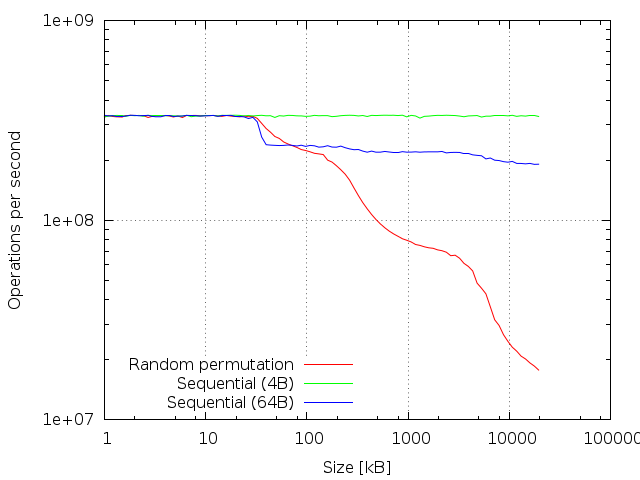
\includegraphics[scale=0.5]{results.png} 
% \end{center}
% \caption{Parallel Monte Carlo integration on Euler compute cluster.}
% \label{fig1}
% \end{figure}

\section{Question 2: MPI Bug Hunt}

\subsection{a)}
There is no MPI code in this snippet. In case the the calculation part was meant to be the 
MPI component, all setup and finalize statements would be missing.

\subsection{b)}
This will cause a deadlock as both rank 0 and rank 1 will first attempt to send their
message with the respective partner not ready to receive. This can be fixed by moving
the \texttt{MPI\_Recv} into the \texttt{if... else} construct and making sure one rank 
first receives and then sends while the other rank first sends and then receives.

\subsection{c)}
If there's only one rank, the program will print \texttt{[0]0} to \texttt{std::cout}.
With more than one rank, the program will also print the above but then hang endlessly, as
\texttt{MPI\_Recv} isn't the proper way to receive broadcast data: If a broadcast is
desired, all ranks should call \texttt{MPI\_Bcast()} and then all ranks end up
with their buffer equal to the buffer of the \texttt{root} argument of the function call.


% \begin{figure}[H]
% \begin{tabular}{ccccc}
% \subfloat[Component 0]{\includegraphics[width = 1.1in]{lin_component_0.eps}} &
% \subfloat[Component 1]{\includegraphics[width = 1.1in]{lin_component_1.eps}} &
% \subfloat[Component 2]{\includegraphics[width = 1.1in]{lin_component_2.eps}} &
% \subfloat[Component 3]{\includegraphics[width = 1.1in]{lin_component_3.eps}} &
% \subfloat[Component 4]{\includegraphics[width = 1.1in]{lin_component_4.eps}} \\
% \subfloat[Component 5]{\includegraphics[width = 1.1in]{lin_component_5.eps}} &
% \subfloat[Component 6]{\includegraphics[width = 1.1in]{lin_component_6.eps}} &
% \subfloat[Component 7]{\includegraphics[width = 1.1in]{lin_component_7.eps}} &
% \subfloat[Component 8]{\includegraphics[width = 1.1in]{lin_component_8.eps}} &
% \subfloat[Component 9]{\includegraphics[width = 1.1in]{lin_component_9.eps}} 
% \end{tabular}
% \caption{10 Principal components of MNIST data set obtained from single linear hidden layer.}
% \label{fig:1}
% \end{figure}




\end{document}